\chapter{Конструкторский раздел}\label{sec:design}
\section{\protect\justifying\protect\RaggedRight Проектирование отношений сущностей}
На рисунке \ref{fig:chen} приведена концептуальная схема проектируемой БД в нотации Чена. 
\begin{center}
	\begin{figure}[H]
		\centering
		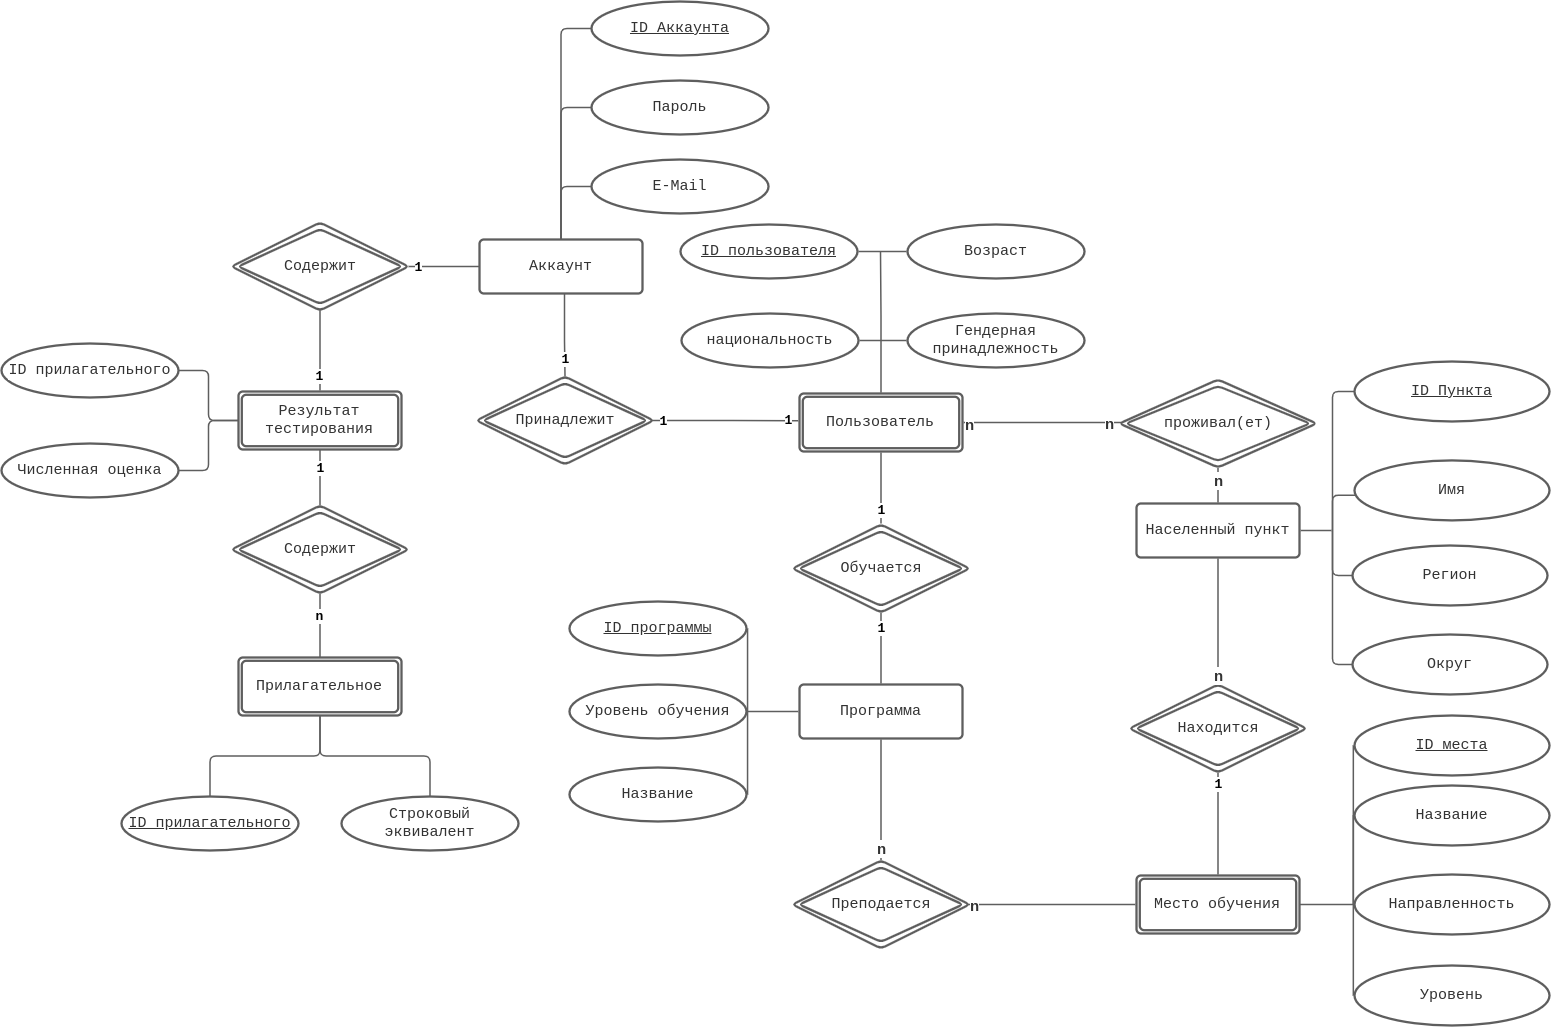
\includegraphics[width=\linewidth]{assets/term-chen.drawio.png}
		\caption{ER-диаграмма сущностей базы данных в нотации Чена}
		\label{fig:chen}
	\end{figure}
\end{center}

Проектируемая база данных ориентирована на хранение информации, получаемой из web-приложения, содержащего систему оценки тональных прилагательных. Функционал приложения должен включать в себя регистрацию, авторизацию и возможность проставления оценок прилагательным. Соответственно, в базе данных можно выделить ряд сущностей. 
\begin{enumerate}
	\item Аккаунт хранит информацию, необходимую при регистрации -- электронная почта и пароль.
	\item Пользователь содержит информацию о личных характеристиках субъекта тональности -- национальность, возраст и гендерная принадлежность. 
	\item Населенный пункт -- это одна из характеристик субъекта тональности. Поскольку пользователь мог менять места проживания, связь этих двух сущностей -- <<многие ко многим>>.
	\item Место обучения -- сущность, содержащая характеристику об образовании, которое получает пользователь.
	\item Результат тестирования включает в себя оценку тонального прилагательного, присвоенная пользователем во время рабочей сессии. Возможные значения оценки -- числа от <<1>> до <<10>>.
	\item Тональное прилагательное.
\end{enumerate} 

\section{Ролевая модель} 
В ролевой модели\cite{Leonard1973} операции, которые необходимо выполнять в рамках какой-либо служебной обязанности пользователя системы, группируются в набор, называемый <<ролью>>.

При использовании ролевой политики управление доступом осуществляется в две стадии: для каждой роли указывается набор полномочий, представляющий набор прав доступа к объектам или частям приложения, затем каждому пользователю назначается его роль.

В разрабатываемой системе выделены три роли, каждой из которых соответствует конкретный функционал системы:
\begin{enumerate}
	\item Опрашиваемому -- функционал регистрации и авторизации, а также прохождения опроса и просмотр его результатов.
	\item Модератору -- функционал просмотра списка всех пользователей системы.
	\item Администратору -- функционал просмотра результатов опроса любого пользователя и общей статистики по опросу.
\end{enumerate}


\section{Нефункциональные характеристики графовых БД}
Зачастую в приложениях, активно использующих операции ввода-вывода, при выполнении одной бизнес-операции происходят массовое чтение и запись связанных между собой данных. В графовых базах данных выполняется несколько операций внутри логического подграфа общего набора данных. Подобное множество можно преобразовать в набор более крупных, тесно связанных операций.

В реляционных базах данных с увеличением размеров и количества данных начинают проявляться недостатки соединения таблиц и ухудшается производительность. Использование смежности без индексов позволяет графовым базам данных перемещаться по сложным соединениям в графе эффективнее, независимо от общего размера набора данных.
\subsection{Нерелевантность внешних кэшей}
Графовые базы данных имеют более высокую эффективность поиска за счет графовой организации хранения данных, благодаря этому разница в скорости доступа к данным в основной СУБД и внешних кэшах незначительна.\cite{Sholichah2020} 

В случае реляционных СУБД кэши используются для выделения <<горячих>>  данных и быстрого обращения к ним. Кэширующие базы данных как правило имеют тип <<ключ-значение>>, реализующие хеш-таблицу, в которой находится уникальный ключ и указатель на конкретный объект данных. Релеватность использования кэшей с реляционными СУБД достигается за счет не только меньшей ассимптотической сложности, но и хранения в данных в оперативной памяти вместо диска, используемого самой СУБД.\cite{aws} Таким образом, из общего набора данных выделяются <<горячие>>, скорость доступа к которым следует по возможности увеличивать. Ассимптотическая сложность алгоритма доступа к данным в графовых СУБД кэш-хранилищ совпадает.
К тому же, использование сторонних кэширующих хранилищ накладывает ограничения на размерность и связанность данных, достаточные, чтобы считать использование их лишенным смысла.

\section{\protect\justifying\protect\RaggedRight Проектирование клиентского приложения}
На рисунке \ref{fig:usecase} представлена диаграмма вариантов использования приложения. 
\begin{center}
	\begin{figure}[H]
		\centering
		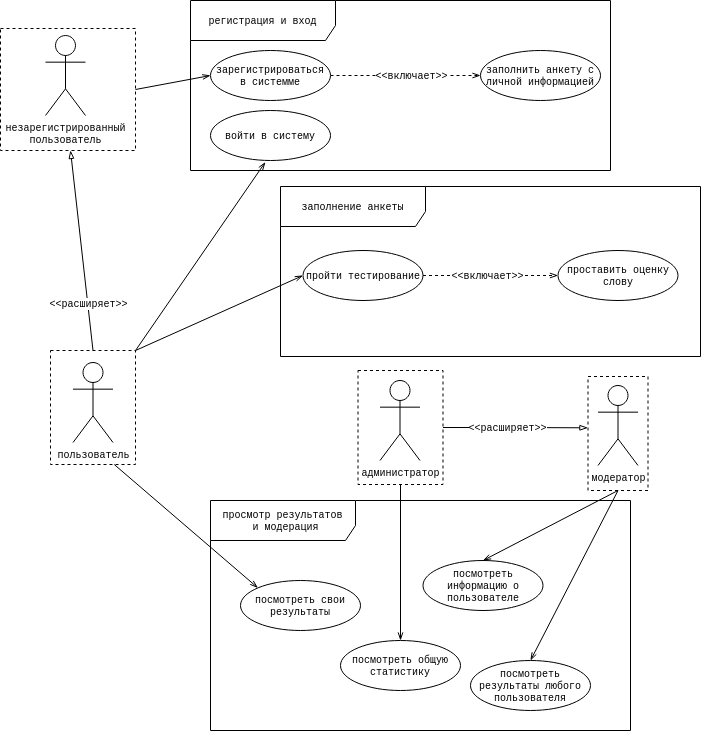
\includegraphics[width=0.85\linewidth]{assets/term-uc.drawio.png}
		\caption{Диаграмма вариантов использования системы}
		\label{fig:usecase}
	\end{figure}
\end{center}
Пользователь системы, имеющий роль <<Модератор>>, может просматривать информацию о всех пользователях, сохраненных в базе данных. Интерфейс пользователя с ролью <<Администратор>> расширяет интерфейс для <<Модератора>> возможностью просматривать общую статистику опроса и результатов всех пользователей.

В случае посещения страниц, для которых у пользователя не соответствующая роль, в интерфейсе отображается соответствующее сообщение и доступ к запрашиваемому функционалу не предоставляется.

Интерфейс незарегистрированного пользователя включает возможность регистрироваться и осуществлять вход в систему. После регистрации или авторизации интерфейс расширяется: опрашиваемый может проходить тестирование и смотреть свои результаты. 

На рисунке \ref{fig:bpmn} представлена модель бизнес-процессов в нотации BPMN.  
\begin{center}
	\begin{figure}[H]
		\centering
		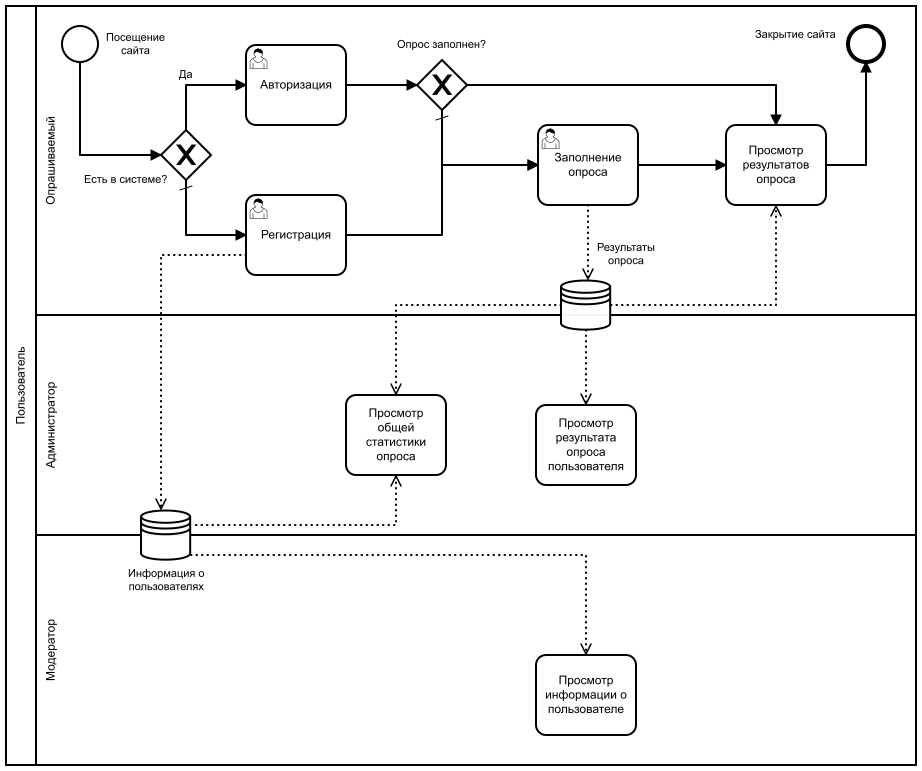
\includegraphics[width=\linewidth]{assets/term-bpmn.png}
		\caption{модель бизнес-процессов в нотации BPMN}
		\label{fig:bpmn}
	\end{figure}
\end{center}
Бизнес-процесс состоит одного пула <<пользователь>>, поделенного на три дорожки -- администратор, модератор и опрашиваемый. Дорожки определяются ролью пользователя, хранимой в базе данных. 

Опрашиваемый посещает сайт и проходит либо регистрацию, либо авторизацию в зависимости от того, был ли он уже зарегистрирован в системе. Далее ему предлагается пройти опрос либо просмотреть результаты в случае если опрос уже пройден. Результаты опроса после его заполнения отправляются в хранилище данных. 

Модератор имеет доступ к части хранилища с информацией о всех зарегистрированных пользователях и может просматривать информацию о любом пользователе. Администратор имеет доступ к результатам и может просматривать общую статистику опроса.

На рисунке \ref{fig:diag1} приведена диаграмма последовательностей для процесса получения результатов опроса от пользователя.

Для заполнения опроса требуется пройти авторизацию. Если пользователь не авторизован, то он получит соответствующее сообщение об ошибке.

При посещении опрашиваемым страницы заполнения опроса на сервер поступает запрос на получение списка прилагательных, которые хранятся в базе данных. Из базы данных список поступает на сервер, затем на клиентское приложение и возвращается пользователю. Пользователь размечает прилагательные, на сервер отправляется список прилагательных с разметкой и результат записывается в базу данных. 

При запросе на просмотр результата на сервере происходит анализ пользовательских данных и сервер отправляет запрос в базу на поиск результата опроса пользователя..

На рисунке \ref{fig:diag2} изображена диаграмма последовательностей для процесса получения полного списка пользователей через защищенную страницу. Выполнять данное действие может только модератор, поэтому перед посещением страницы происходит проверка прав пользователя, отправившего запрос. 

\begin{center}
	\begin{figure}[H]
		\centering
		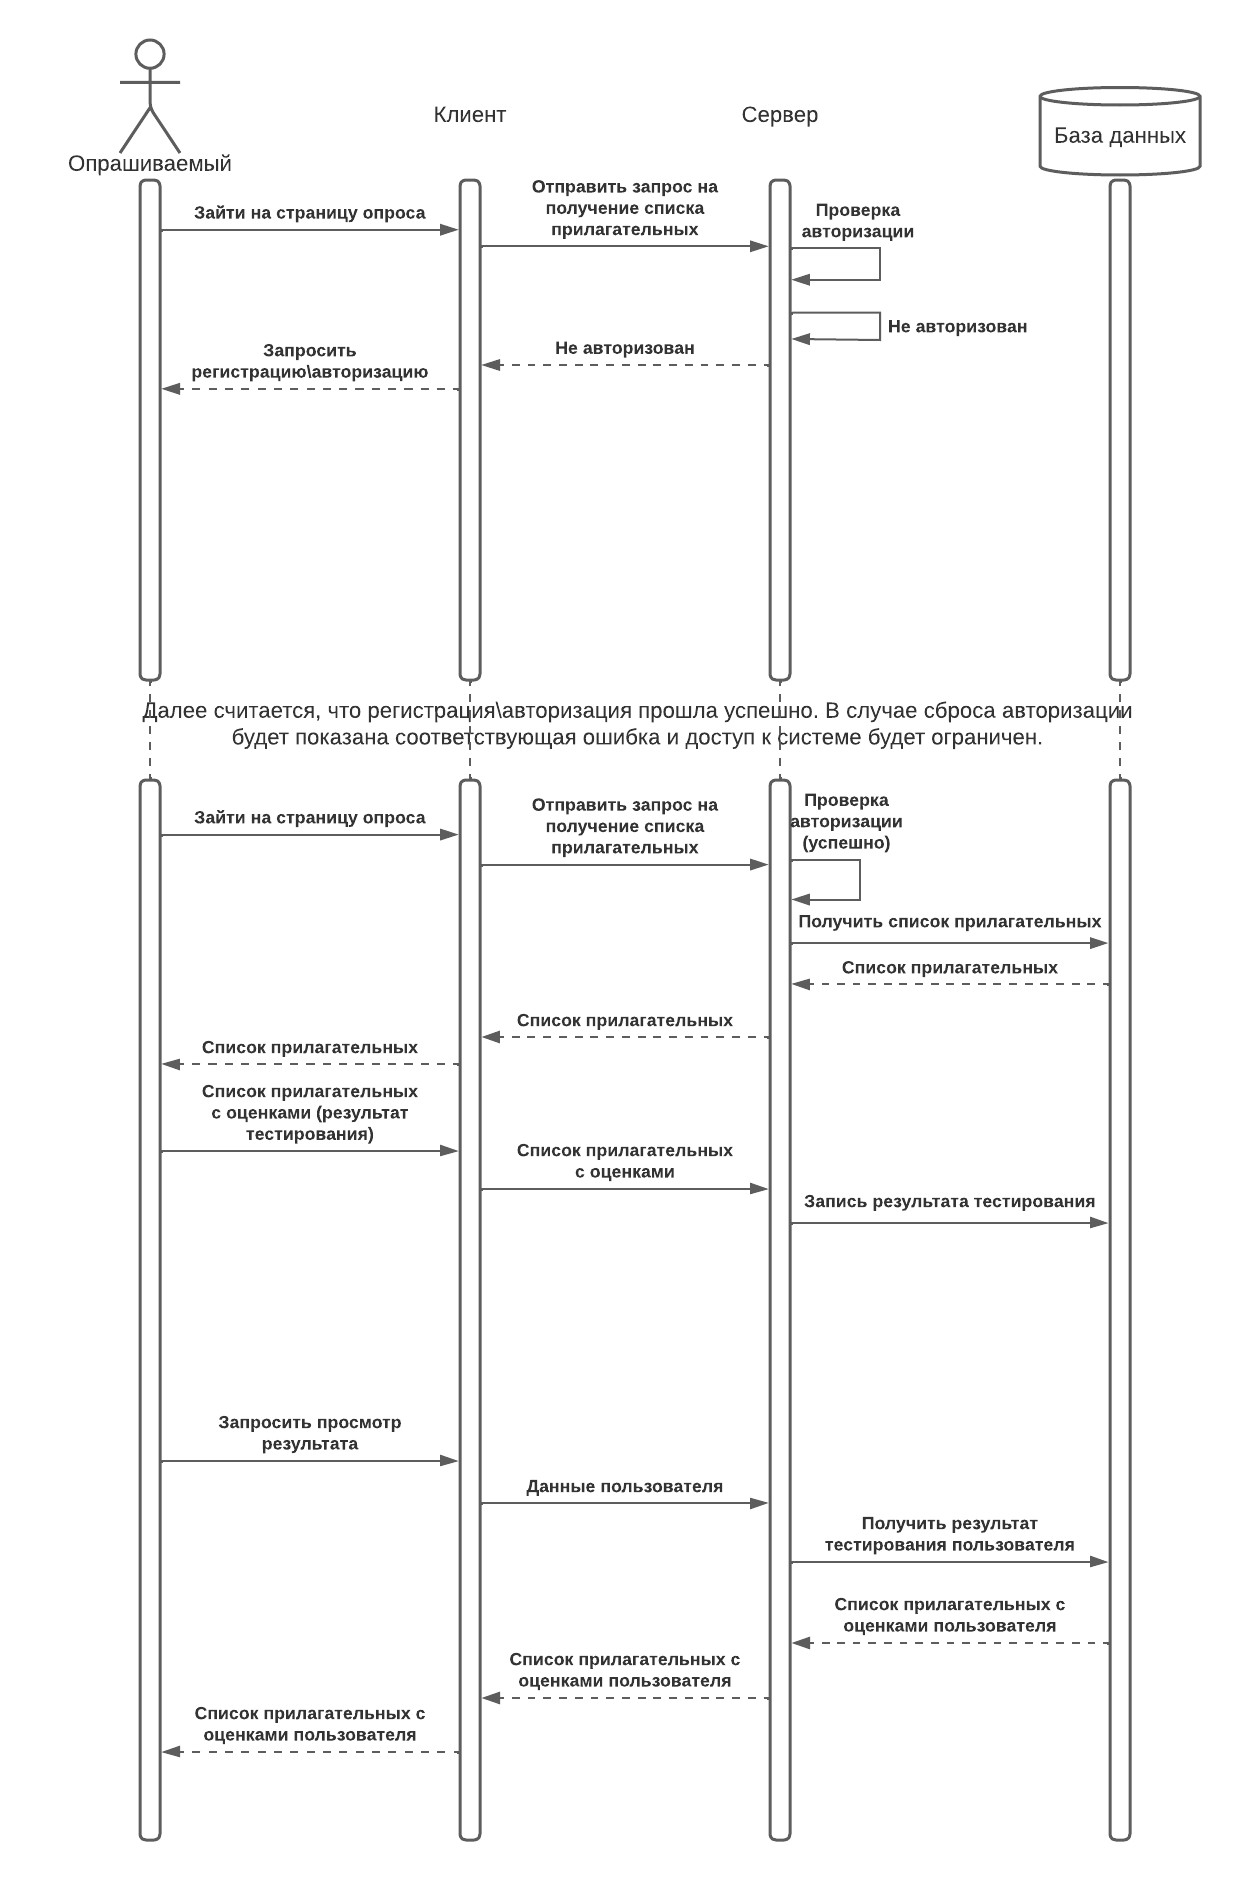
\includegraphics[width=\linewidth]{assets/diag-1.png}
		\caption{Диаграмма последовательностей для процесса получения результатов опроса от пользователя}
		\label{fig:diag1}
	\end{figure}
\end{center}

\begin{center}
	\begin{figure}[H]
		\centering
		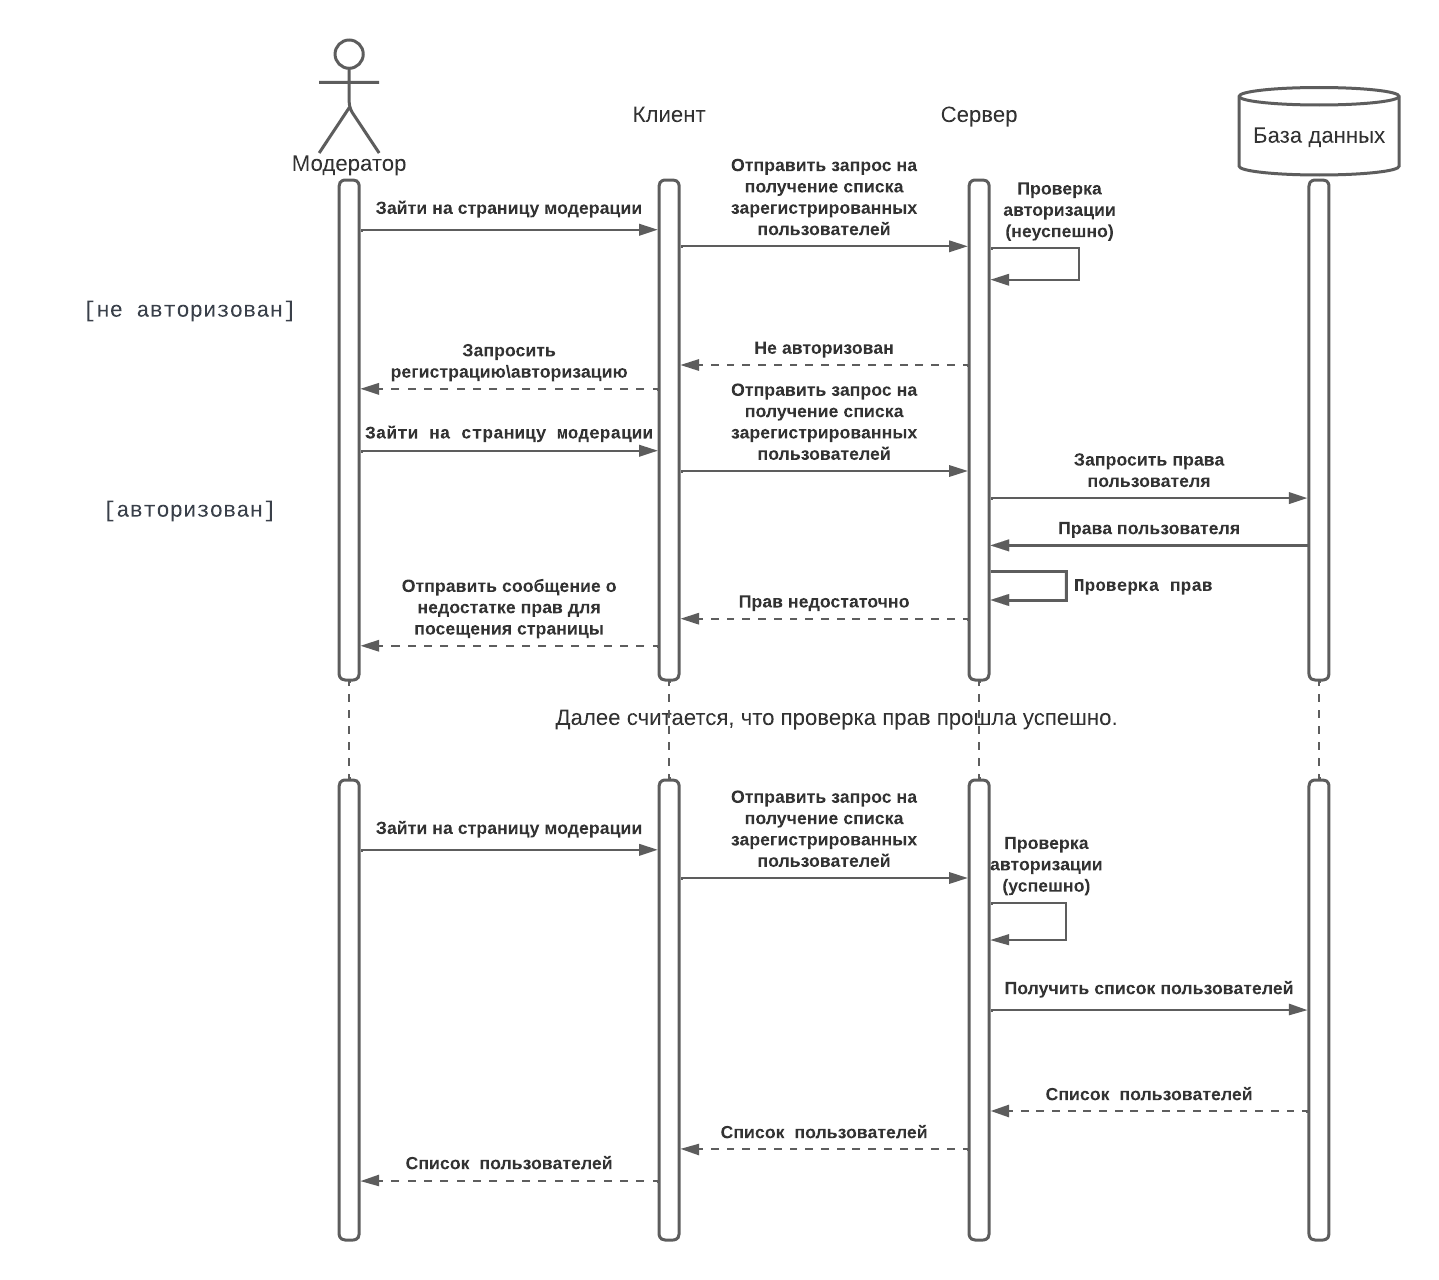
\includegraphics[width=\linewidth]{assets/diag-2.png}
		\caption{Диаграмма последовательностей для процесса получения списка зарегистрированных пользователей}
		\label{fig:diag2}
	\end{figure}
\end{center}

На рисунке \ref{fig:diag3} изображена диаграмма последовательностей для процесса получения статистики опроса через защищенную страницу. Выполнять данное действие может только администратор, поэтому перед посещением страницы происходит проверка прав пользователя, отправившего запрос. 

\begin{center}
	\begin{figure}[H]
		\centering
		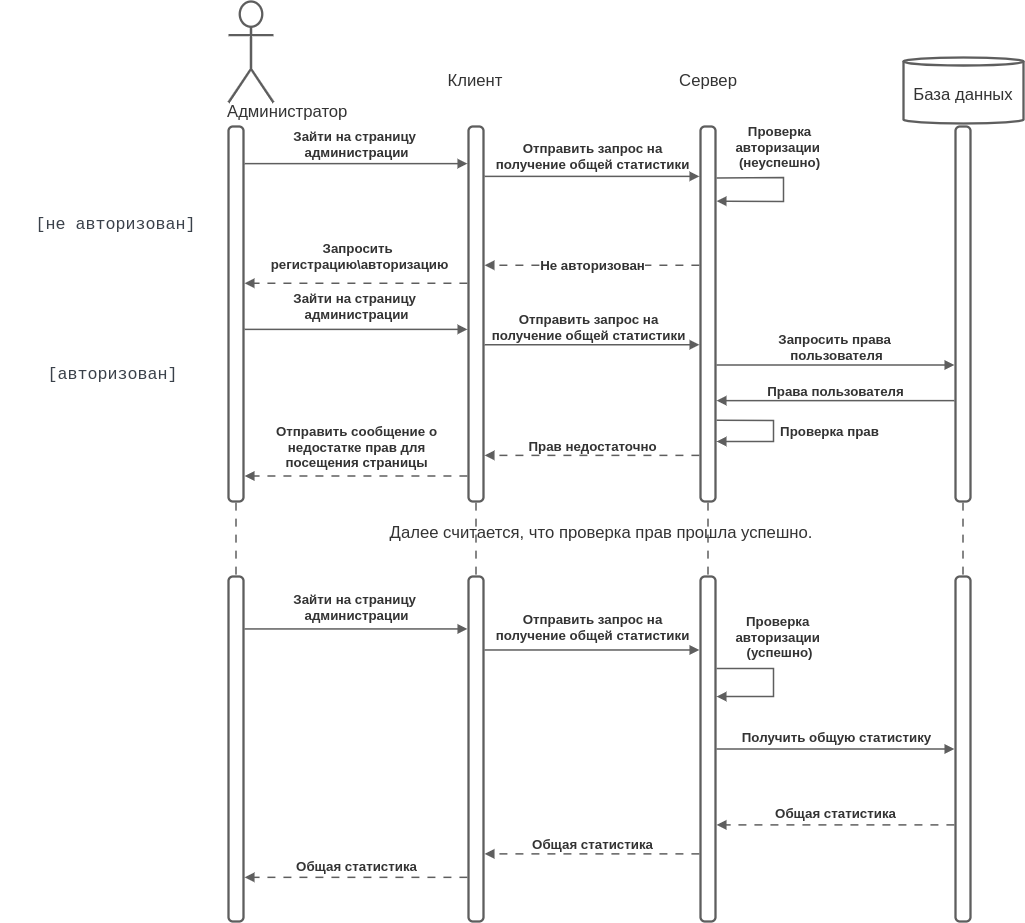
\includegraphics[width=\linewidth]{assets/diag-final.png}
		\caption{Диаграмма последовательностей для процесса получения общей статистики опроса}
		\label{fig:diag3}
	\end{figure}
\end{center}

\addsec{Вывод}
Проектируемая база данных хранит информацию, получаемую из web-приложения, содержащего систему оценки тональных прилагательных. В базе выделен соответствующий ряд сущностей, приведенный на рисунке \ref{fig:chen}. Для базы выделено три роли: <<Опрашиваемый>>, <<Модератор>> и <<Администратор>>, каждая из которых соответствует дорожке пула <<пользователь>>, присутствующей в бизнес-процессе (рисунок \ref{fig:bpmn}). 

Использование сторонних кэширующих хранилищ накладывает ограничения на размерность и связанность данных, достаточные, чтобы считать использование их лишенным смысла -- графовые базы данных имеют более высокую эффективность поиска за счет графовой организации хранения данных.


